% -*- root: ../../main.tex -*-
\section{View}
\label{sec:view_design}

L'\textbf{interfaccia grafica} rappresenta uno degli elementi di spicco per quanto riguarda l'\textbf{aspetto visivo} di un videogioco. Gli utenti finali, infatti, non saranno interessati tanto alla progettazione del gioco quanto al modo con cui esso si presenta.

Al fine di garantire un'\textbf{aspetto gradevole} al gioco si è deciso quindi di puntare verso un \textbf{design modulare} che permettesse di poter definire in modo chirurgico l'intera \textbf{user experience}.

\subsection{Struttura a Schermate}
Il sistema di presentazione è stato così scomposto in \textbf{schermate multiple} (\texttt{Screen}) delegando ad ognuna di esse un particolare aspetto dell'\textbf{interazione con l'utente}.

\begin{figure}[H]
	\centering
	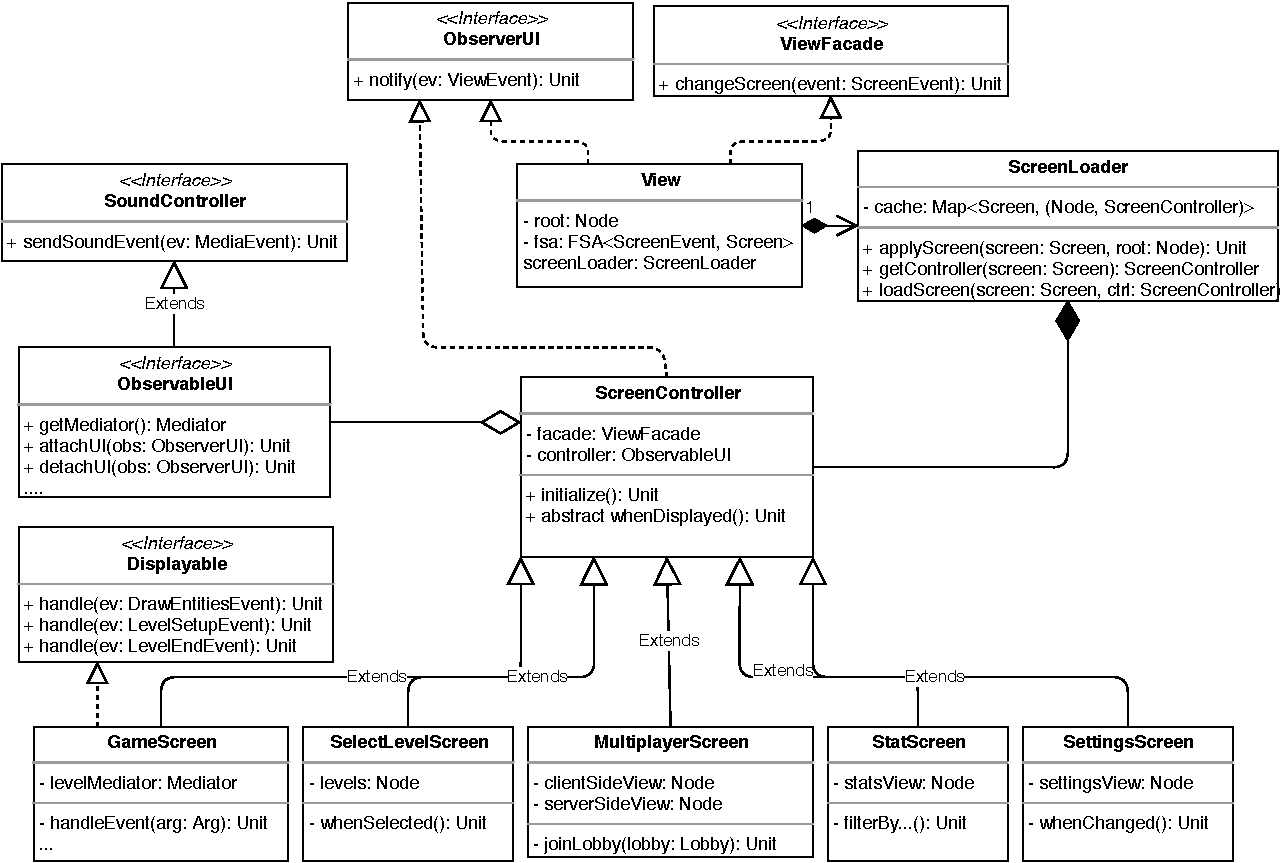
\includegraphics[width=0.99\columnwidth]{drawio/viewFacade/viewFacade.pdf}
	\caption{Diagramma delle classi relativo all'implementazione del pattern façade.}
	\label{fig:viewFacade}
\end{figure}

Come vediamo in \ref{fig:viewFacade} sono presenti cinque schermate fondamentali:
\begin{itemize}
	\item{\textbf{GameScreen:}}
	Costituisce il cuore dell'interazione con \textbf{ECS} ed è il luogo in cui prende vita il vero e proprio \textbf{gameplay}. Come già anticipato in \ref{sec:mediator_design}, questa schermata avrà la capacità di collegarsi in modo lasco con il \texttt{Mediator} e agirà da \textbf{Input/Output} di \textbf{eventi} (\texttt{SendCommand} \texttt{DrawEntities}).
	\item{\textbf{SelectLevelScreen:}}
	Rappresenta una delle poche \textbf{schermate innestate dinamicamente} nell'esperienza di gioco e il suo scopo consiste essenzialmente nella \textbf{scelta} dei vari \textbf{livelli disponibili}. 
	\item{\textbf{MultiplayerScreen:}}
	È qui dove la logica del multiplayer prende vita. L'utente che vorrà giocare con questa modalità non dovrà fare altro che portarsi in questa schermata e selezionare la \textbf{modalità di gioco} \\ (\texttt{client/server-mode}) da utilizzare.
	\item{\textbf{StatScreen:}}
	È una semplice schermata relativa alle statistiche di gioco. Come in ogni \textbf{arcade} che si rispetti, questa mostrerà una lista dei \textbf{migliori punteggi} correlati al giocatore corrispondente.
	\item{\textbf{SettingsScreen:}}
	Ogni gioco necessita di una serie di impostazioni al fine di garantire una \textbf{buona usabilità} e \textbf{personalizzazione}. Questo aspetto sarà presente e sarà posizionato in una schermata dedicata. 
\end{itemize}

\paragraph{ScreenController:}
Un dettaglio che potrebbe far storcere il naso risiede nel fatto che ogni schermata \textbf{estende} da un'unica classe \texttt{ScreenController}. Que-sto dettaglio dipende fortemente dalla tecnologia utilizzata in fase di implementazione, \texttt{JavaFx}. In \texttt{JavaFx}, infatti, ad ogni layer di presentazione (\texttt{fxml}) è associato un \textbf{modulo di controllo} chiamato, appunto, \texttt{ScreenController}. Ogni \texttt{ScreenController} deve possedere la capacità di interfacciarsi con il \\ \texttt{Controller} e come vedremo dovrà allo stesso modo poter \textbf{interagire} con le altre \textbf{schermate}.

\subsection{Il pattern Façade}
Il \textbf{pattern Façade} si configura come una soluzione davvero interessante al \textbf{problema di interazione} tra schermate introdotto precedentemente. Un \textbf{façade} (facciata) consiste in un oggetto che permette, attraverso un'\textbf{interfaccia più semplice}, l'\textbf{accesso a sottosistemi} che espongono \textbf{interfacce complesse} e \textbf{molto diverse tra loro}. 

Nella situazione mostrata precedentemente, il façade (\texttt{ViewFacade}) permette di poter \textbf{gestire l'interazione} con ogni sotto-schermata da \textbf{qualsiasi schermata} mostrata in un certo istante all'utente. Questo permette alle sotto-schermate di poter essere \textbf{sostituite} in un unico modo garantendo così il \textbf{Single Responsability Principle}. Il pattern inoltre permette di elevare un insieme di \textbf{metodi comuni} all'interno di un'\textbf{unica interfaccia} permettendo così di rispettare il principio \textbf{DRY}.

\paragraph{Façade e MVC:}
L'oggetto façade proposto (\texttt{ViewFacade}) implementa interamente il contratto definito per l'interfaccia grafica (\texttt{View}); di conseguenza esso rappresenta a tutti gli effetti il modulo di \textbf{View} all'interno del pattern architetturale \texttt{MVC}.

\paragraph{Façade e gestione delle schermate:}
Poiché il \texttt{ViewFacade} rappresenta un \textbf{accesso} disponibile \textbf{a tutte le sotto-schermate}, esso deve poter accedere a tutta la \textbf{logica} relativa alle stesse. Per garantire maggiori performance di caricamento si è deciso di costruire un \textbf{modulo} dedicato al \textbf{loading} e al \textbf{caching} delle \textbf{schermate}: lo \texttt{ScreenLoader}. 

Il funzionamento è molto semplice: quando viene richiesta una schermata essa viene \textbf{cercata nella cache}, nel caso in cui non sia presente allora verrà \textbf{caricata} e successivamente \textbf{mostrata all'utente}. È importante che la \textbf{cache} di alcune schermate particolari (\texttt{GameScreen}) venga \textbf{invalidata} al fine di garantire una \textbf{dinamicità del contenuto}.


